\newpage
\section{Implementierung}

Zur Simulation einer zuvor gemessenen Linsenverzerrung wurde in pbrt eine neue Kameraklasse \texttt{DistortionCamera} hinzugefügt. Die vorliegende Implementierung unterstützt drei rein radiale Verzerrungsmodelle, die von der Datenbank des Lensfun-Projektes\cite{lensfun_basic} (Version 0.3.2\footnote{Zum Zeitpunkt der Abgabe war diese die aktuellste stabile Version von Lensfun}) unterstützt werden. Lensfun ist eine Open-Source Softwarebibliothek, die eine Datenbank vermessener Kameras und Linsen sowie Funktionen zur Korrektur von Linsenverzerrungen, chromatischen Aberrationen und Vignettierung bereitstellt.

\subsection{Verzerrungsmodelle in der Lensfun-Datenbank}

Die in Lensfun implementierten Modelle bilden rein \emph{radiale} Linsenverzerrungen ab, wie in Abschnitt \ref{subsec:verzerrungsmodelle} beschrieben. Dazu wird eine Funktion $f:[0,1] \rightarrow R$ definiert\footnote{Der tatsächliche Wertebereich der Funktionen hängt von ihren Parametern ab (siehe \ref{subsubsec:modeldef}). Diese werden durch Messung an realen Kameras ermittelt. Typische Werte sorgen dafür, dass der Wertebereich zwischen 0 und 1 liegt, was im Kontext eines normierten Radius sinnvoll ist (siehe \ref{subsubsec:norm_radius}).}, die den unverzerrten Radius auf den verzerrten Radius abbildet. Dabei wird in einem normalisierten Koordinatensystem gearbeitet.

\subsubsection{Koordinatensystem und Normalisierung}
\label{subsubsec:norm_radius}

Der Radius wird definiert als der normierte Abstand vom Bildmittelpunkt. Dieser wird standardmäßig als $p_m = (\frac{x_{res}}{2}, \frac{y_{res}}{2})$ angenommen, wobei $x_{res}$ und $y_{res}$ die Bildauflösung in x- bzw. y-Richtung bezeichnen. In der Datenbank kann auch eine gemessene Abweichung von diesem "idealen" Bildmittelpunkt angegeben werden. Wir behandeln zunächst den Fall, dass keine Abweichung gegeben ist, bzw. die Abweichungen in x- und y-Richtung null betragen. Die Normierung erfolgt so, dass die halbe Bilddiagonale $r_e$ die Länge eins hat. Da diese den größten Radius im Bild darstellt, ist dadurch immer $r \in [0,1]$ (siehe Abbildung \ref{fig:norm}). 

\begin{figure}[h]
	\centering
	\begin{tikzpicture}
	%Bildumriss
	\draw[thick] (0,0) -- (8,0) -- (8, -4) -- (0,-4) -- (0,0);
	%Bildmitte
	\draw (4,-2) circle [radius=0.02] node[above] {$p_m$};
	%Koordinatenystem
	\draw[semithick, gray, ->] (0,0) -- (1,0) node[above] {$x$};
	\draw[semithick, gray, ->] (0,0) -- (0,-1) node[left] {$y$};
	%Eckenradius
	\draw[-{Latex[length=3mm]}] (4,-2) -- (8,0);
	%Radius Beschriftung
	\node[]	 at (6, -0.7) {$r_e$};
	%Beschriftung Bilddimensionen
	\node[left] at (0,0.2) {$(0,0)$};
	\node[left, red] at (0,-0.2) {$(0,0)$};
	\node[right] at (8,-3.8) {$(x_{res}, y_{res})$};
	\node[right, red] at (8,-4.4) {$(\frac{x_{res}}{r_e}, \frac{y_{res}}{r_e})$};
	\node at (4, -2.5) {($\frac{x_{res}}{2}, \frac{y_{res}}{2})$};
	\node[red] at (4, -3.2) {($\frac{x_{res}}{2 r_e}, \frac{y_{res}}{2 r_e})$};
	\end{tikzpicture}
	
	\caption{Verwendete Normalisierung der Bildkoordinaten nach \cite{imatest, lensfun}. Das Koordinatensystem wurde in Übereinstimmung mit \cite[S. 359]{pbrt_book} gewählt. Pixelkoordinaten in schwarz, normalisierte Koordinaten in rot.	\label{fig:normalisation}}
	\label{fig:norm}
\end{figure}

Die Transformation von Pixelkoordinaten zu normalisierten Koordinaten besteht einfach in einer Division durch $r_e$. Dies lässt sich einfach nachvollziehen, indem der Radius (in Pixelkoordinaten) für einen der Eckpunkte berechnet wird:
\begin{equation}
	r_e = \sqrt{(x_{eck} - x_{mitte})^2 + (y_{eck} - y_{mitte})^2} = \sqrt{\overline{x}^2 + \overline{y}^2}
\end{equation}
Skaliert man nun alle Koordinaten mit einem Faktor $k$, so ist der skalierte Eckenradius
\begin{equation}
	r_s = \sqrt{(k \overline{x})^2 + (k \overline{y})^2} = \sqrt{k^2 (\overline{x}^2 + \overline{y}^2)} = k r_e.
\end{equation}
Um $r_s = 1$ zu erfüllen, muss dann $k = \frac{1}{r_e}$ gelten.

Im Fall, dass eine Abweichung der optischen Achse vom Bildmittelpunkt ungleich null vorliegt, stellt sich für die Normalisierung das Problem, dass nun der maximal mögliche Radius nicht mehr durch die halbe Bilddiagonale gegeben ist, sondern durch den Abstand von $p_m$ zur am weitesten entfernten Ecke. Mit welcher Ecke dann $r_e$ berechnet werden muss, hängt von den Vorzeichen der Abweichungen $x_{a}$ und $y_{a}$ ab. Anschließend erfolgt die Normalisierung wie oben beschrieben. Die gemessenen Werte für $x_{a}$ und $y_{a}$ werden in der Lensfun-Datenbank ebenfalls normalisiert gespeichert, wobei die Skalierung dadurch definiert wird, dass die kleinere Bilddimension gleich 2 gesetzt wird. Die entsprechenden Pixelwerte können also durch
\begin{equation}
\begin{pmatrix}
x_{a,pixel} \\ y_{a,pixel}
\end{pmatrix}
 = \frac{\min\{x_{res}, y_{res}\}}{2} \cdot
 \begin{pmatrix}
 x_{a,norm} \\ y_{a,norm}
 \end{pmatrix}
\end{equation} 
berechnet werden.

\newpage
\subsubsection{Modelldefinitionen}\label{sec:Modeldefinitions}
\label{subsubsec:modeldef}

Im Folgenden steht $r_u$ immer für den normierten unverzerrten Bildradius, der durch eine Verzerrungsfunktion $f$ auf den verzerrten Radius $r_d$ abgebildet wird. Diese Bezeichnungen und die Definitionen der Verzerrungsfunktionen sind der Dokumentation von Lensfun entnommen \cite{lensfun}.

\textbf{Poly3:} Das Poly3-Modell besteht aus einem Polynom dritter Ordnung mit einem Parameter $k_1$. Es gilt unabhängig von $k_1$ immer $f(0) = 0$ und $f(1) = 1$. Dadurch, dass nur ein Parameter vorhanden ist, eignet sich das Modell vornehmlich zur Modellierung weniger komplexer Verzerrungen.
\begin{equation}
	f_{poly3}(r_u) = r_u \cdot (1 - k_1 + k_1 r_u^2)
\end{equation}

\textbf{Poly5:} Dieses Modell verwendet ein Polynom fünfter Ordnung und kann dadurch komplexere Verzerrungen nachbilden als das Poly3-Modell. Es wird dafür ein weiterer Parameter benötigt. Anders als beim Poly3-Modell ist hier nicht $f(1) = 1$ garantiert.
\begin{equation}
	f_{poly5}(r_u) = r_u \cdot (1 + k_1 r_u^2 + k_2 r_u^4)
\end{equation}

\textbf{PTLens:} Dieses Modell wurde aus der PTLens-Datenbank, auf der das Lensfun-Projekt aufbaut, übernommen. Das Modell besteht aus einem Polynom vierter Ordnung, mit drei Parametern $a,b,c$ und ist so aufgebaut, dass wieder die Normierung $f(1) = 1$ gilt.
\begin{equation}
	f_{ptlens}(r_u) = r_u \cdot (a r_u^3 + b r_u^2 + c r_u + 1 - a - b - c)
\end{equation}

\subsection{Implementierung}\label{subsec:implementation}

Die Klasse \texttt{DistortionCamera} implementiert die Linsenverzeichnung. Dabei werden die Richtungen der ausgesandten Strahlen relativ zum "Referenzmodell Lochkamera" modifiziert, sodass die Verzeichnung durch die unperfekte Linse im gerenderten Bild sichtbar wird (vgl. Abschnitt \ref{sec:DistortionRaytracer}). Der Raytracer ruft zum Erzeugen der Strahlen die Methode \texttt{GenerateRay} auf. Dies passiert für jeden Pixel des zu erzeugenden Bildes mindestens einmal\footnote{Der verwendete Sampler gibt vor, wie häufig und auf welche Art und Weise für ein Pixel Strahlen generiert werden.}. Die Berechnung der Strahlrichtung in Abhängigkeit der betrachteten Pixelkoordinaten erfolgt also in \texttt{GenerateRay}.

Damit ergibt sich für die Implementierung die Anforderung, dass bei einer vorgegebenen Verzerrungsfunktion $f$ vor Beginn des Renderings die inverse Funktion bestimmt werden muss. Da für die in der Lensfun-Datenbank verwendeten Modelle keine einfache analytische Inverse gefunden werden kann, wird ein numerischer Ansatz verfolgt. Dazu werden zunächst Werte von $f$ für eine Reihe von $r_i$ im erlaubten Bereich bestimmt. Die Inverse wird dann als Polynom mittels des Least Squares Verfahrens angenähert.


\subsubsection{Least Squares}
\label{subsubsec:least}

Die Methode der kleinsten Quadrate (engl.: \emph{Least Squares}, kurz LS) stellt ein Verfahren, zu einer gegebenen Menge an Punkten eine Funktion zu finden, die eine mögliche unbekannte Gesetzmäßigkeit hinter der Lage der Punkte annähert \cite{lsq_wolfram}.

Sei $P = \{(x_1, y_1), (x_2, y_2), ..., (x_n, y_n)\}$ die Menge der bekannten Punkte mit $x_i, y_i \in R$. Man nimmt nun an, dass zwischen x und y ein funktionaler Zusammenhang bestehe, der durch $m$ reelle Parameter $a_j$ bestimmt wird. Damit lässt sich $y_i = f(x_i; \overrightarrow{a})$ schreiben, wobei $\overrightarrow{a} \in R^m$ die Parameter zusammenfasst. LS versucht nun, den unbekannten Parametervektor so zu ermitteln, dass die Summe der quadratischen Abweichungen $S^2$ minimiert wird:
\begin{equation}
\begin{split}
\overrightarrow{a} \in \argmin_{\overrightarrow{a} \in R^M} \{ S^2 \}, \quad
S^2 =  \sum_{i=1}^{N} (y_i - f(x_i, \overrightarrow{a}))^2
\end{split}
\label{eq:opt}
\end{equation}
Setzt man für $f$ ein Polynom vom Grad $k$ an, so ist $m = k+1$ und
%\begin{equation}
\begin{gather}
f(x_i, \overrightarrow{a}) = a_0 + a_1 x_i + \dots + a_k x_i^k = \sum_{j = 0}^{k} a_j x_i^j %\\
\end{gather}
%\end{equation}
Für das Minimum müssen die partiellen Ableitungen nach allen Parametern null sein.
\begin{equation}
\frac{\partial S^2}{\partial a_l} = -2 \sum_{i=1}^{n}(y_i - a_0 + a_1 + \dots + a_k x^k) x^l = 0, \quad 0 \leq l \leq m
\end{equation}
Es muss also ein Gleichungssystem gelöst werden, dass sich wie folgt darstellen lässt:
\begin{gather}
X^T X \cdot \overrightarrow{a} = X^T \cdot
\overrightarrow{y} \label{eq:solution}
\end{gather}
mit 
\begin{gather}
X =
\begin{bmatrix}
1 & x_1 & \dots & x_1^k \\
1 & x_2^k & \dots & x_2^k \\
\vdots & \vdots & \ddots & \vdots \\
1 & x_n & \dots & x_n^k
\end{bmatrix}
\text{und} \overrightarrow{y} = \begin{bmatrix}
y_1 \\ y_2 \\ \vdots \\ y_n
\end{bmatrix}
\end{gather}
Sind alle $x_i$ paarweise voneinander verschieden, so ist $X^T X$ regulär. Damit ist das Problem unter dieser Bedingung immer eindeutig lösbar. Die Matrixgleichung \ref{eq:solution} kann somit numerisch oder direkt durch Finden von $(X^T X)^{-1}$ gelöst werden \cite{lsq_poly_wolfram}. In der Implementierung von \texttt{DistortionCamera} geschieht dies mittels LR-Zerlegung (beschrieben zum Beispiel in \cite{bronstein}).

Ist also eine Funktion $f(x)$ gegeben, so kann durch Auswahl von $n$ paarweise unterschiedlichen Werten $x_i$ im Bereich $[0,1]$ die Menge $P = \{ (x_1, y_1), (x_2, y_2), \dots, (x_n, y_n) \}, \quad y_i = f(x_i)$ erzeugt werden. Um nun die inverse Funktion $g(x) = f^{-1}(x)$ per LS anzunähern, tauscht man in den Paaren in $P$ jeweils $x_i$ und $y_i$ und führt dann das LS Verfahren wie oben beschrieben durch. Dies entspricht dem Optimierungsproblem
\begin{equation}
\begin{split}
\overrightarrow{a} \in \argmin_{\overrightarrow{a} \in R^m} \{ S^2 \}, \quad
S^2 =  \sum_{i=1}^{n} (x_i - f(y_i, \overrightarrow{a}))^2\quad.
\end{split}
\end{equation}
Im Vergleich zu Gleichung \ref{eq:opt} sind also die Rollen von $x_i$ und $y_i$ getauscht.

\subsubsection{Anwenden des Modells}
\label{subsubsec:anwenden}

Sind die Parameter für $g$ bestimmt, kann damit $p_1$ aus $p_2$ bestimmt werden (vgl. Abbildung \ref{fig:model}). Da die implementierten Modelle rein radial arbeiten, muss zunächst zu $p_2 = (x_2, y_2)$ der Radius $r_2$ bestimmt werden (die Koordinaten sind hierbei und im Folgenden die nach \ref{subsubsec:norm_radius} normalisierten Koordinaten):
\begin{equation}
r_2 = \sqrt{ (x_2 - x_{mitte})^2 + (y_2 - y_{mitte})^2 }
\end{equation}
Der Radius $r_1$ des Punktes $p_1$ wird dann mit 
\begin{equation}
r_1 = g(r_2)
\end{equation}
bestimmt. Zum Berechnen der Koordinaten von $p_1$ ist es hilfreich, einen radialen Einheitsvektor $\overrightarrow{e_r}$, der vom Bildmittelpunkt zum betrachteten Punkt $p_2$ zeigt, zu definieren:
\begin{equation}
\overrightarrow{e_r} = \begin{pmatrix} x_2 - x_{mitte} \\ y_2 - y_{mitte} \end{pmatrix} \cdot \frac{1}{r_2}
\end{equation}
Damit ergeben sich die Koordinaten von $p_1$ zu 
\begin{equation}
\begin{pmatrix} x_1 \\ y_1\\ \end{pmatrix} = 
\begin{pmatrix} x_{mitte} \\ y_{mitte} \end{pmatrix} + 
\overrightarrow{e_r} \cdot r_1 =
\frac{r_1}{r_2} \cdot
\begin{pmatrix} x_2 \\ y_2 \end{pmatrix} + 
\begin{pmatrix} x_{mitte} \\ y_{mitte} \end{pmatrix} \cdot
\frac{r_1}{r_2}
\end{equation}

\subsubsection{Umsetzung in C++}
Die Implementierung von \texttt{DistortionCamera} ist in den Dateien \texttt{distortion.h} und \linebreak \texttt{distortion.cpp} enthalten. \texttt{DistortionCamera} erbt dabei von \texttt{ProjectiveCamera} (siehe Abbildung \ref{fig:uml}).

\begin{figure}[h]
	\begin{minipage}{.5\textwidth}
		\centering
		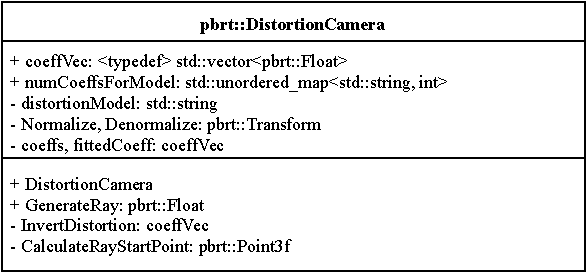
\includegraphics[height=.4\columnwidth]{uml_distortioncam}
	\end{minipage}
	\begin{minipage}{.5\textwidth}
		\centering
		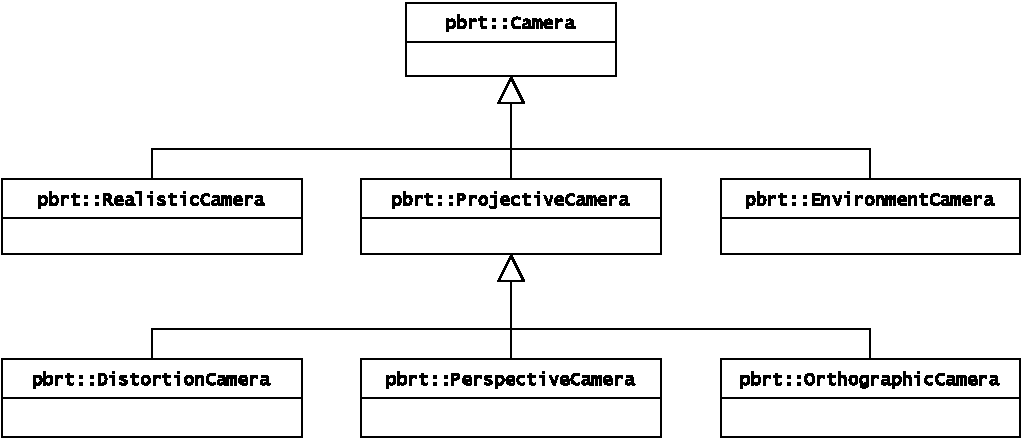
\includegraphics[height=.4\columnwidth]{uml_classes}
	\end{minipage}
	\caption{UML-Darstellung von \texttt{DistortionCamera} (links) und Einordnung in die Klassenstruktur der vorhandenen Kameraklassen (rechts).}
	\label{fig:uml}
\end{figure}

Im Konstruktor der Klasse wird zunächst eine Validierung des übergebenen Verzerrungsmodells durchgeführt. Ist kein Modell in der zu rendernden Szene definiert, so wird die inverse Verzerrungsfunktion zu $f(r) = r$ gesetzt. Das Rendering entspricht dann dem einer \texttt{PerspectiveCamera}. Anschließend wird überprüft, ob das zu übergebende Modell implementiert ist und die korrekte Anzahl an Koeffizienten übergeben wurde. Dies geschieht anhand der Variablen \texttt{numCoeffsForModel}. Sind die Eingabeparameter korrekt, wird per LS die inverse Verzerrungsfunktion angenähert.

%\begin{figure}
%	\centering
%	\includegraphics[scale=0.75]{flowchart}
%	\caption{Validierung des übergebenen Modells}
%\end{figure}

Außerdem wird im Konstruktor die Transformation \texttt{Normalize} definiert (siehe \ref{subsubsec:norm_radius}), sowie die dazugehörige inverse Transformation \texttt{Denormalize}.
\newpage
\begin{lstlisting}[caption={Transformation zur Normalisierung der Pixelkoordinaten}]
/* -------- Define transformations for ray generation --------*/
Float xRes = film->fullResolution.x;
Float yRes = film->fullResolution.y;
Float cornerRadius = sqrt(pow(xRes/2, 2) + pow(yRes/2, 2)) / 2.;
NormalizeToCornerRadius = Scale(1. / cornerRadius, 1. / cornerRadius, 1.);
Denormalize = Inverse(NormalizeToCornerRadius);
\end{lstlisting}

Zum Bestimmen der inversen Verzerrungsfunktion ist in \texttt{distortion.h} die Funktion \texttt{fitPolyCoeffs} implementiert. Diese setzt das Least Squares Verfahren wie in Abschnitt \ref{subsubsec:least} beschrieben um.

Für die Matrizenoperationen wird auf Funktionen aus der Boost-Bibliothek zurückgegriffen. Boost ist eine Sammlung von Open Source C++-Bibliotheken \cite{boost}. In diesem Fall wird die Unterbibliothek \texttt{Boost::numeric::uBLAS} verwendet \cite{ublas}. BLAS steht dabei für "Basic Linear Algebra Subprograms", was Inhalt und Zielsetzung der Bibliothek gut zusammenfasst. Zusätzlich ist eine Funktion \texttt{evalPolynomial} vorhanden, die für einen gegebenen Satz an $m$ Polynomkoeffizienten $a_i$ und einen Wert $x \in R$ die Funktion $y = a_0 + a_1 x + a_2 x^2 + \dots + a_{m-1} x^{m-1}$ berechnet. In \texttt{InvertDistortion} wird die übergebene Verzerrungsfunktion abgetastet und anschließend der Koeffizientenvektor der inversen Funktion genähert.
\begin{lstlisting}[caption={"Abtasten" des Verzerrungsmodells und Invertierung}]
// fill sample vector according to the model used
for (int i = 0; i < sampleSize; i++) {
	x[i] = i / scale;
	y[i] = (*modelFunc)(x[i], coeffs);
}
coeffVec polyCoeffs = fitPolyCoeffs(y, x, polyDegree);
\end{lstlisting}

Zur Erzeugung des Strahls für ein vom Sampler übergebenes \texttt{CameraSample} wird dann \texttt{CalculateRayStartpoint} in \texttt{GenerateRay} aufgerufen. \texttt{CalculateRayStartpoint} berechnet den Ausgangspunkt des Strahls für den im aktuellen \texttt{CameraSample} übergebenen Punkt auf dem Bildsensor, wie in \ref{subsubsec:anwenden} beschrieben. Die Funktion \texttt{GenerateRay} unterscheidet sich von ihrem Äquivalent in \texttt{PerspectiveCamera} nur durch die folgende Zeile:
\begin{lstlisting} [caption={Anpassung in der Methode \texttt{GenerateRay}}]
Point3f pCamera = RasterToCamera(CalculateRayStartpoint(sample));
\end{lstlisting}

Neben dieser eigentlichen Implementierung der neuen Kameraklasse waren noch geringe Anpassungen nötig, um die Parameter für \texttt{DistortionCamera} aus einer \texttt{.pbrt}-Datei zu parsen. Diese betrafen die Funktion \texttt{MakeCamera} in \texttt{/src/core/api.cpp}. Außerdem musste die neue Abhängigkeit von der Boost-Bibliothek in \texttt{CMakeLists.txt} eingepflegt werden.

Soll in Zukunft ein neues Verzerrungsmodell in die Klasse eingebaut werden, so sind folgende Punkte zu erledigen:
\begin{itemize}
	\item Mögliche neue Parameter müssen in der Funktion \texttt{MakeCamera} aus der Szenenbeschreibung geparsed werden und im Konstruktor von \texttt{DistortionCamera} hinzugefügt werden.
	\item Der Name des neuen Modells und die benötigte Anzahl von Koeffizienten müssen in der Variablen \texttt{numCoeffsForModel} hinzugefügt werden.
	\item Eine Funktion, die die Modellberechnung durchführt, muss implementiert werden. Die bisherigen Modellfunktionen sind als \texttt{inline} Funktionen in \texttt{distortion.h} implementiert worden.
	\item Schließlich muss die Modellfunktion in \texttt{InvertDistortion} ausgewählt werden, wenn das neue Modell übergeben wird.
\end{itemize}

\subsection{Interface in der Szenenbeschreibung}

Die \texttt{DistortionCamera}-Klasse übernimmt alle Argumente von der \texttt{PerspectiveCamera}. Diese sind in \cite{pbrt_file} bereits dokumentiert. Zusätzlich können folgende Argumente übergeben werden:
\begin{table}[h]
	\begin{tabularx}{\textwidth}{l|l|l|X}
		\textbf{Datentyp} & \textbf{Name} & \textbf{Default} & \textbf{Beschreibung} \\ \hline \hline
		String & model & NO\_MODEL & Name des Verzerrungsmodells. Momentan sind verfügbar: "poly3lensfun", \mbox{"poly5lensfun"}, "ptlens".\\
		Float & coefficients & [0, 1] & Koeffizientenvektor für das gegebene Verzerrungsmodell. \\
		Float & centerx & 0.0 & Verschiebung des Bildmittelpunkts in \mbox{x-Richtung} \\
		Float & centery & 0.0 & Verschiebung des Bildmittelpunkts in \mbox{y-Richtung}
	\end{tabularx}
\end{table}